\documentclass{llncs}
\usepackage{graphicx}        % standard LaTeX graphics tool
                             % when including figure files
\usepackage{url}
%%%%%%%%%%%%%%%%%%%%%%%%%%%%%%%%%%%%%%%%%%%%%%%%%%%%%%%%%%%%%%%%%%%%%%%%%%%%%%%%%%%%%%%%%
\usepackage{subfigure}
\usepackage{amsmath}

\begin{document}
\sloppy

\title{Increasing Performance via Gamification in a Volunteer-Based Evolutionary Computation System}
\titlerunning{Increasing Performance via Gamification in a Volunteer
  EC System}


\author{anonymous author name \inst{1} \and anonymous author name\inst{2} \and  anonymous author name \inst{1}}

\institute{anonymous institution, some city, country
\and
anonymous institution, some city, country\\
\email{example@example.edu}\\
\email{example2@example.edu}}



%\author{Mario Garc\'ia-Valdez\inst{1} \and Juan J. Merelo Guerv\'os\inst{2} \and  Lucero Lara \inst{1}}

%\institute{Instituto Tecnol\'ogico de Tijuana, Tijuana BC, Mexico
%\and
%Universidad de Granada, Granada, Spain
%\email{mario@tectijuana.edu.mx}\\
%\email{jmerelo@geneura.ugr.es}}

%\authorrunning{Garc\'ia-Valdez, Merelo, \& Lara }

\maketitle


\begin{abstract}

Distributed computing systems can be created using volunteers; these
are users who spontaneously, after receiving an invitation, decide to
provide their own resources or storage to contribute to a common
effort. They can, for instance, run a script embedded in a web page;
thus, 
collaboration is straightforward, but also ephemeral, with resources
depending on the amount of time the user decides to lend. This  implies that 
the user has to be kept engaged so as to obtain as many computing cycles as
possible. In this paper, we analyze a volunteer-based evolutionary computing system called
% NodIO
Anonymous with the objective of discovering design decisions that encourage volunteer
participation, thus increasing the overall computing power. We present the results of
an experiment in which a gamification technique is applied by adding a leader-board
showing the top scores achieved by registered contributors. In the
% NodIO
Anonymous system volunteers can
participate without the need to create an account, so one of the
questions we wanted to address was
if the need to register would have a negative impact on user participation.
The experiment results show that even if only a small percentage of users created an account,
those participating in the competition provided around 90\% of the
work, thus effectively increasing the performance of the overall
system. 

\keywords{Distributed Evolutionary Algorithms, Volunteer Computing,
  Socio-Technical Systems}
\end{abstract}

\section{Introduction}

The world wide web is an increasingly reliable and high-performance
operating system for running distributed applications. Besides the
maturity of HTTP, the underlying protocol itself, there are other
factors: the JavaScript virtual machine embedded in every browser
and the REST interface, providing a {\em de facto} standard interface for
communication. A distributed system based on the browser can be
created easily using these mechanisms, which have lately been enhanced
by WebSockets for lower latency; you can gather users by just
announcing the URL. This approach for creating distributed experiments is called {\em
  volunteer}, {\em cycle-scavenging}, or {\em opportunistic} computing
\cite{sarmenta2001volunteer} and it dates back, in different shapes
and underlying mechanisms, to the origin of the Internet
\cite{david-seti:home}.

In this context, we are mainly interested in evolutionary algorithms
\cite{milani2004online,sherry2012flex,jj-ppsn98}%,
% population-based search and optimization methods inspired by
% the theory of Evolution and its molecular basis.
. The fact that they are population-based makes them suitable for a
straightforward distribution of work to different clients, and since
they have an asynchronous nature, there is no considerable impact on
their performance, and might even be beneficial for a number of
reasons, including increased diversity
\cite{cantu-paz:migration-policies}. All these properties make them
ideal candidates for volunteer computing setups such as the one
presented in this paper, at least if some minimal changes are made to
the usual sequential or parallel algorithms that rely on a static
setup. 

But even if adaptation is straightforward, there are several open issues in the research regarding the
application of volunteer computing techniques to the development of
distributed evolutionary algorithms of which the most important is
approaching the problem as a socio-technical system
\cite{vespignani2009predicting,merelo2015designing}, which integrates
user decisions and behavioral patterns in the model; this
includes trying to optimize the number of users or the overall time
they contribute in a particular
experiment. The challenge is to design a system that, whatever the
number of users available and willing to perform the experiment, it is able to
maximize their contribution to the evolutionary algorithm. One obvious
way of achieving that is trying to find as many users as possible. But
another approach, and the one that we will be following in this paper, is
to delve into the socio-technical nature of the system, using
gamification techniques to try and improve the amount of time every user will
lend to the system. However, there is a tradeoff with gamification,
since users have to be identified in some way to participate, and thus
it has to include some way of user authentication,
which is a hurdle that might take users away; however, the open design
of the system we use means that we can actually mix anonymous-non
gamified and authenticated-gamified users, with only the small overhead
of adding the gamification mechanism.

This trade-off between ease of use, allowing users to
participate by just visiting a web page, and personalization, making
registration compulsory and subsequently authenticate in order to
participate, is what we will analyze in this paper. In a sociotechnical system such as this one, every
decision the user has to take has an influence on the overall
performance, and registration could be seen as a hurdle to volunteers
trying to participate in an ephemeral experiment, so it is a challenge
to analyze what actually happens in this case; quite clearly, the
inclusion of gamification techniques has an impact on page loading and
complexity of server-side programming; if eigher the number of users
or the amount of time they contribute to the experiment is not enough,
it would be better to revert to the purely anonymous system.

The rest of the paper is organized as follows: Next we will briefly
present the state of the art in opportunistic distributed evolutionary
computation (EC). Section \ref{sec:gamification} will describe the
framework and the problem used in the experiments, which are publicly
available under a free license. The results of each of the steps in the incremental design are presented in Section
\ref{sec:experiments}, to finally wrap up with the conclusions.



\section{Related Work}
\label{sec:soa}

Volunteer computing involves users who decide to run a program that acts
as a client or as a peer in a distributed computing experiment
and, as such, has been deployed in many different ways from the
beginning of the Internet, starting with the SETI@home framework for
processing extraterrestrial signals \cite{david-seti:home}, or a
high-throughput queuing system such as HTCondor \cite{HTCondor}.
However,
the dual facts of the introduction of JavaScript as a universal language for the
browser and the browser itself as both an ubiquitous web and Internet client has
made this combination the most popular for volunteer computing
frameworks such as the one we are using here, and whose first version
was described in \cite{DBLP:conf/gecco/GuervosG15}. Systems based on the
JavaScript/browser combination
emphasize the ephemerality, ease of use, and universality, while
systems such as HTCondor or BOINC might be more adequate for work that % citation for BOINC (?)
requires higher availability of volunteer resources. In order to increase availability, systems rely on downloadable clients, and in some cases like HTCondor, they also require administrative access to certain resources.

Several authors have already described systems using JavaScript either
for unwitting
\cite{unwitting-ec,boldrin2007distributed,apolonia2012enhancing} or volunteer
\cite{langdon:2005:metas,gecco07:workshop:dcor} distributed
evolutionary computation and it has been used by several
authors ever since. More recent efforts include
\cite{duda2013distributed,DBLP:journals/corr/abs-0801-1210,EvoStar2014:jsEO,martinez2015capataz,pan2015gray}. In fact, this last paper \cite{pan2015gray} performs an analysis of what is called {\em Gray computing} covering aspects of
feasibility, cost-effectiveness, change in the user\'s experience and the
architectural optimization needed, concluding that the computing power
available is vast and it can be cost-effective to use it.

The SPACE framework \cite{leclerc2016seamless}, using a peer to peer approach, distributes fitness evaluations across a heterogeneous pool of cloud compute nodes and volunteer computers running a browser. In SPACE, peers establish a bi-directional communication with the server using the \texttt{Socket.io} JavaScript library.
As an experiment they provide an \texttt{ASM.js} compiled version of the RoboGen software platform, showing that JavaScript can be used in a broad
spectrum of applications.

Recent works have been using crowdsourcing in order to train robots
for human interaction, a representative work of this trend is that of
Anetsberger \& Bongard \cite{anetsbergerrobots} in which they propose
training simulated robots for the grounding of language symbols. They do this by using human observers that issue arbitrary commands to these robots via the web, providing positive or negative reinforcement to the resulting actions of the robot. For interaction, they use the Twitch streaming platform at which users can issue commands through the
platform\'s integrated chat service. Subjects were incentivized to
interact with the system by GUI features that provided participants
with a sense of involvement with the simulation. This kind of system
could add additional dynamics, because users can collaborate or
even compete with each other when issuing their commands. This approach has been called {\em social cloud} \cite{6404452}, emphasizing the fact that user participation is gamified in order to obtain the most from it \cite{7027564}.

The proof-of-concept efforts described above, do not go any further than trying to find out how many users join the effort, and how many of them the system can support. In fact, systems such as the one described in
\cite{gecco07:workshop:dcor} had severe scaling issues; some of them
also tried to find out how much time was needed to find the solution
or, alternatively, how many users would be needed to be competitive
against single-user single-computer implementations of the same
algorithm. Lately, researchers have tried to integrate volunteer computing techinques as a part of a larger distributed computing effort \cite{leclerc2016seamless}.  In fact, systems using volunteers exclusively, exhibit a certain amount of unpredictability, and they might be better used in combination with ready-available computing power.

As indicated in the introduction, the human is an integral part of the system, which we can consider a human computation {\em human computation} \cite{quinn2011human}. Giving the user more control, and adding visibility to their participation might have positive effects. In fact, the BOINC project applies this technique by having a web page presenting the ``Top 100 multi-project BOINC participants'' in which the name of the volunteer, the number of projects, GFLOPS, country and team are displayed
(\url{https://boinc.berkeley.edu/chart_list.php}).

Next we will present the gamification technique used in this experiment.

\section{Gamification}
\label{sec:gamification}
A definition given by Huotari  \cite{huotari2012defining} is ``Gamification is
the process by which gaming concepts are brought to real world tasks associated with
real people''. Gamification uses game design elements out of the domain of games
with the objective of enhancing the user\'s experience, engagement, productivity,
learning, among others. Deterding et al. proposes the following definition:
 ``Gamification” is the use of game design elements in non-game contexts''
 \cite{deterding2011gamification}.

Gamification techniques in a volunteer context seeks to persuade
users to use their natural desire to compete, learn and socialize in
given non-game context application \cite{deterding2011game,hamari2014does}.
Some works give a form of reward to users, these include
points \cite{sutter2010browse}, achievement badges or levels \cite{hamari2011framework},
the filling of a progress bar \cite{o2010get}, or providing the user with virtual currency.
By Making the rewards for  tasks achievements visible to other players or
providing leader boards are ways of encouraging players to compete \cite{hickman2010total}. In this work, a leader board was implemented in order to promote competition, presenting only the all-time top five participating users. Competition can also have problematic consequences, which can result in
negative conduct, low cooperation and collaboration, or disadvantaging certain player demographics
such as women \cite{kumar2013gamification}. Another gamification technique
is to make existing tasks feel more like games \cite{deterding2010just}.
Some techniques used in this approach include adding meaningful choice,
on-boarding with a tutorial, increasing challenge, and adding narrative \cite{mcgonigal2011reality}.



\begin{figure*}[htb]
    \centering
        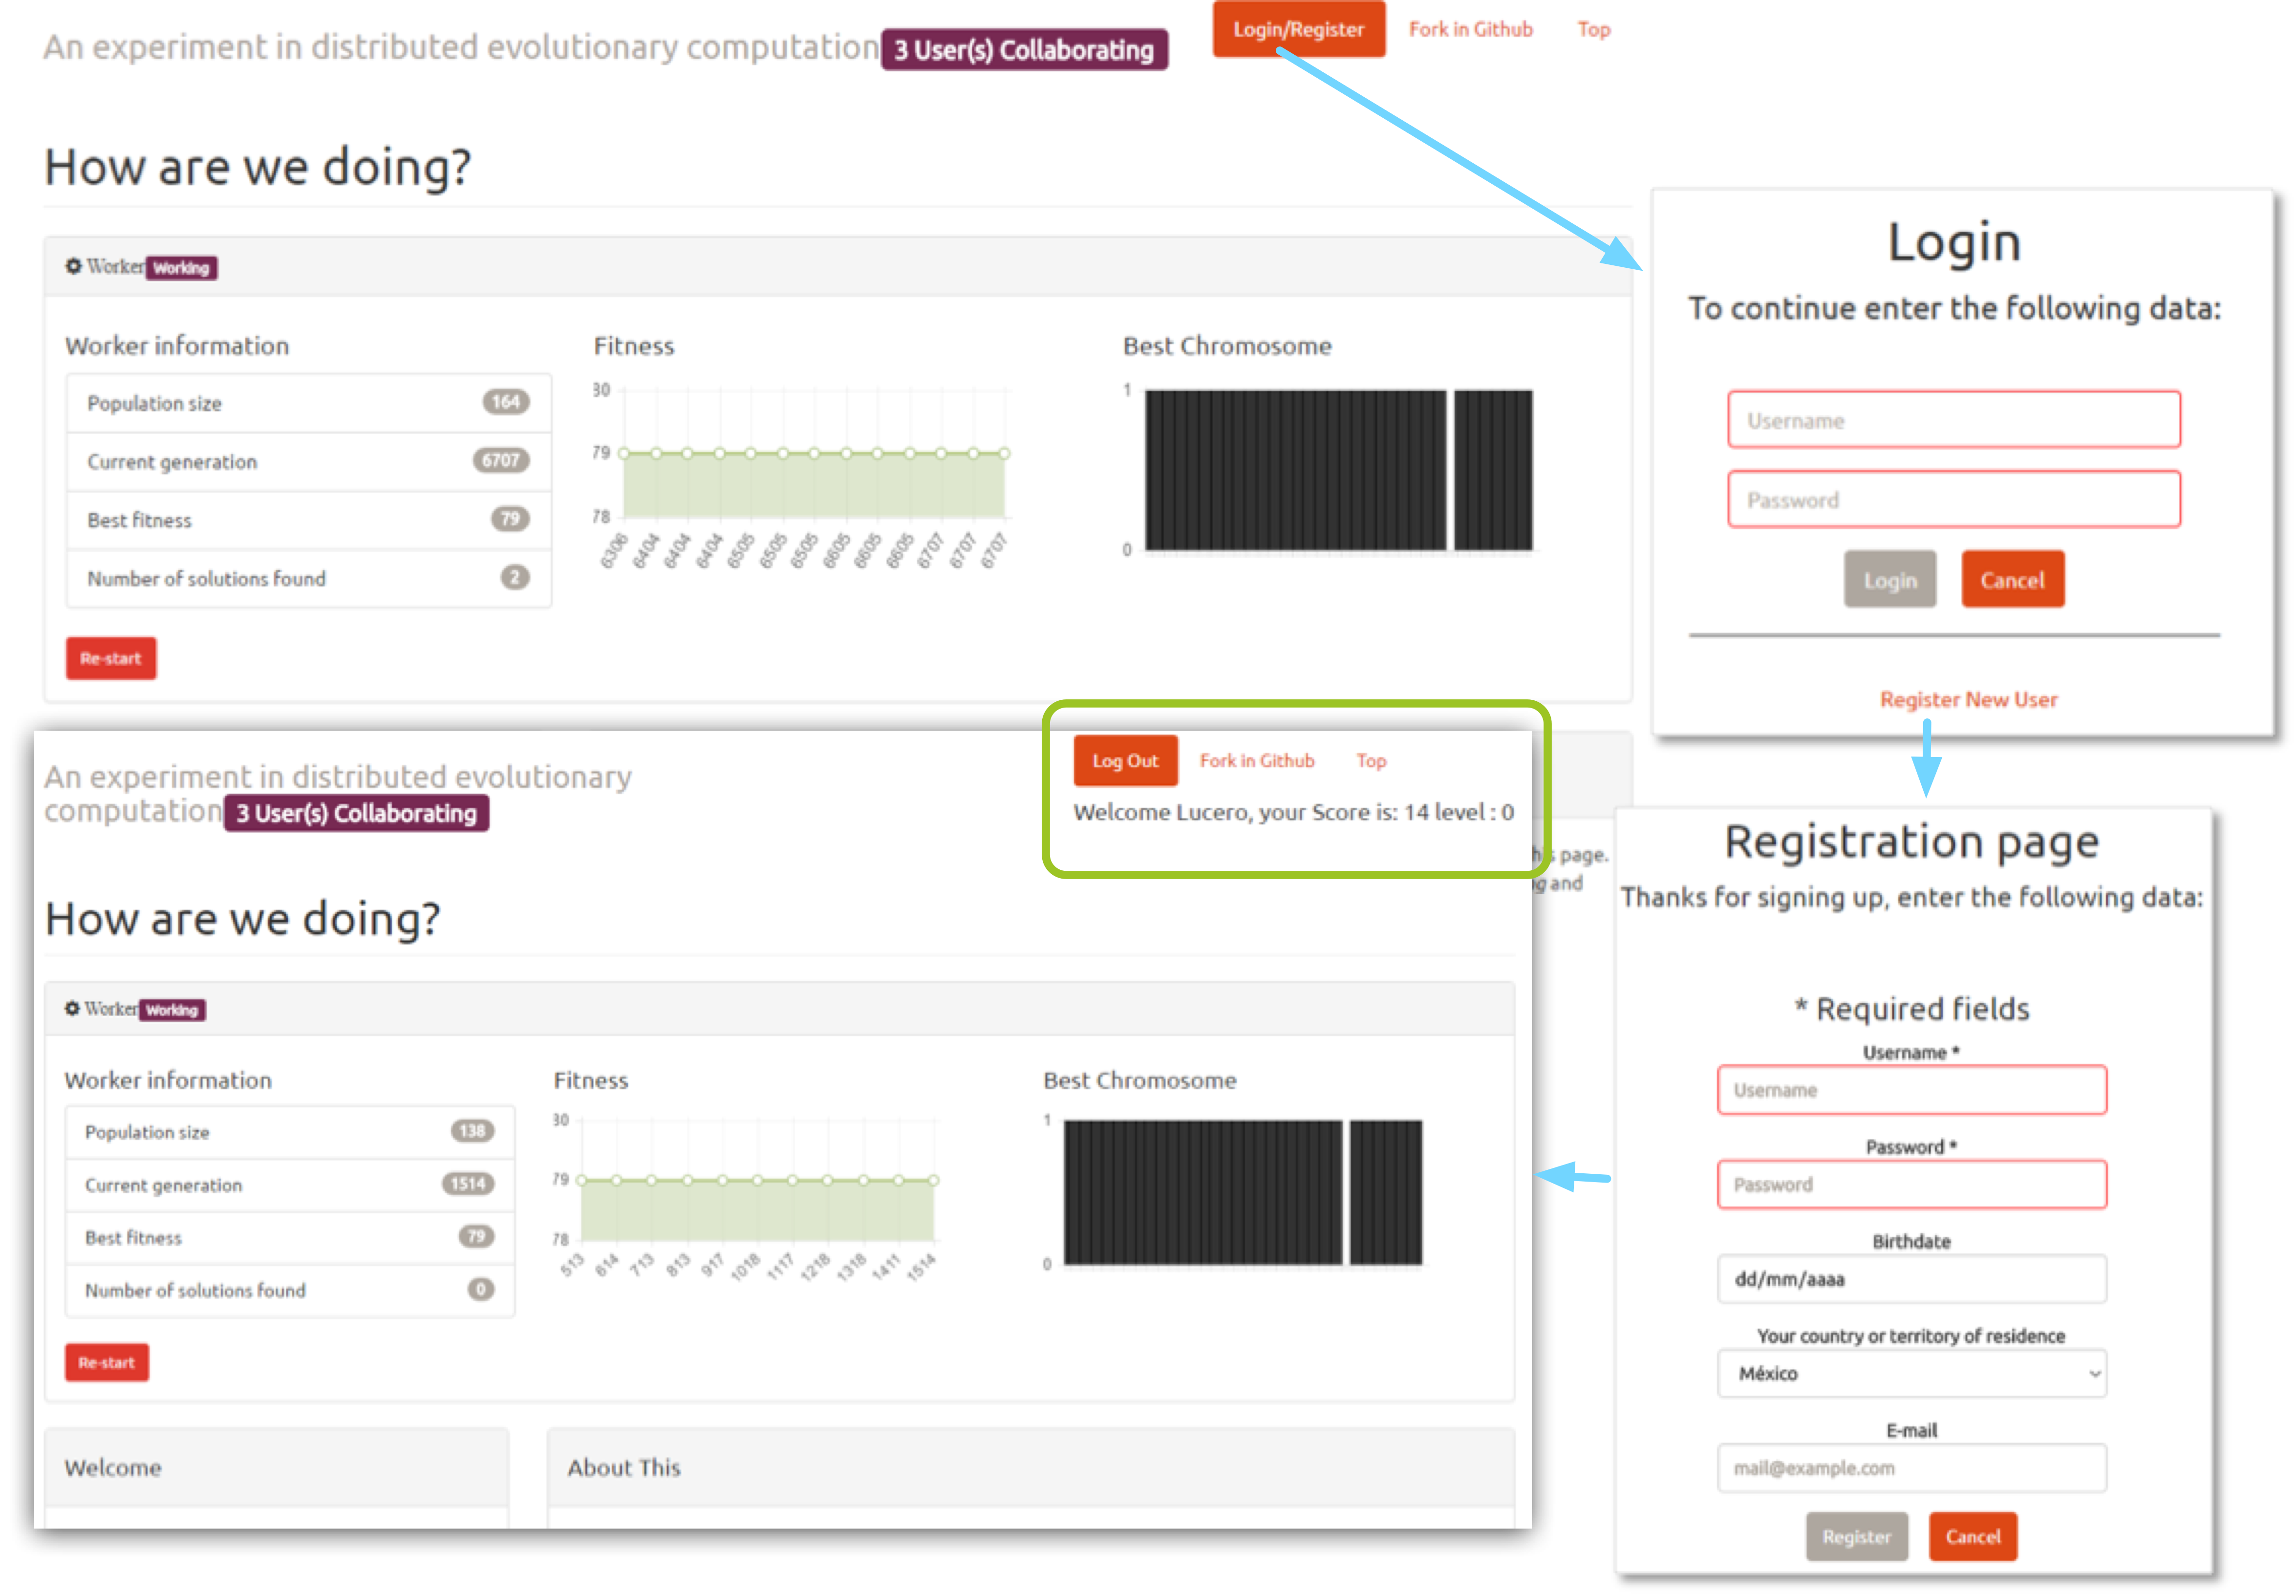
\includegraphics[width=5in]{img/login.png}
    \caption{ User interface: Landing page, and Log-in and registration dialogs.
    }
    \label{fig:login}
\end{figure*}

\section{Experiment}
\label{sec:experiments}

In this experiment a gamification technique is applied to
the Anonymous
% {\sf NodIO}
volunteer computing framework, using the
particular version described in \cite{DBLP:conf/gecco/MereloCGCRV16,2016arXiv160101607M}.
The objective of the experiment is to test the kind of impact
applying a gamification technique has on user engagement in this
particular application. In order to apply a rewarding system
user authentication had to be developed first. In earlier designs
this functionality was not desired because it was seen as a barrier
for participation. After all, the advantage of a browser based volunteer system
is precisely the minimum amount of user intervention needed to start.
The last thing a user wants to see is yet another registration form.
Then, the first design decision for this version is that registration is optional and simple as shown in Figure \ref{fig:login}.

The gamification technique employed in this work is based on a rewarding mechanism
\cite{dubois2013understanding}. In general rewards  consist of a reputation system
with score points, levels and leader boards. Points are awarded to users in response of
the accomplishment of certain activities that need to be encouraged. In these case
a point is awarded for each PUT sent to the server. Levels are a long
term achievement, in this case the level depends on the score:
\[ \text{level}(\text{score};a,b)=
    \begin{cases}
      0,                                    &  \text{score}\leq a\\
      2(\frac{\text{score}-a}{b-a})^{2},    &  a\leq \text{score}\leq \frac{a+b}{2}\\
      1-2(\frac{\text{score}-b}{b-a})^{2},  & \frac{a+b}{2} \leq \text{score}\leq b\\
      1,                                    & \text{score}\geq b
   \end{cases}
\]
The function returns a normalized value that is multiplied by the maximum level
in this case 100. The variables $a$=100 and $b$=7360 are set to give users a rapid increase of
levels at the beginning; this function is represented in Figure \ref{fig:s}.
%
\begin{figure*}[htb]
    \centering
        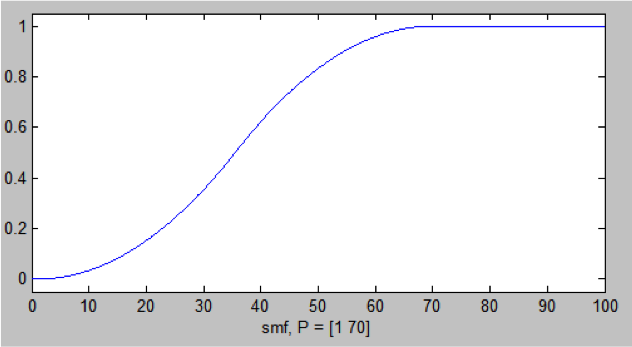
\includegraphics[width=3in]{img/s.png}
    \caption{$S$ function used to assign the user's level.
    }
    \label{fig:s}
\end{figure*}

After login, registered users are welcomed by their name, and they can see
their current score and level. All users can see in a modal dialog the leader board.
While the modal is opened, the scores are refreshed every second. All other
functionality is available to all users and is the same as the previous
%{\sf NodIO}
Anonymous version, showing the state of the current algorithm.
In the front page a link to the open source code of the experiment was also
available \url{https://undisclos.ed}
% \url{https://github.com/lucero21/login-master}


\subsection{Problem}
In the browser, each page visiting the experiment loads an HTTP Web Worker
that runs a local island of an evolutionary algorithm to solve a
multi-modal problem called {\em l-trap} which has been used extensively
as a benchmark for evolutionary algorithms and is represented in figure \ref{fig:trap},  \cite{fernandes2009using,nijssen2003analysis}.
This function counts the number of bits in a sequence $l$ and assigns
the local maximum $a$ if it has 0 bits and the global maximum $b$ if it has $l$
bits, this makes the fitness fall into a {\em trap}
as the number of bits increases, and decreasing linearly until a change in slope
is reached at point $z$, adding a deceptive component for evolutionary algorithms. In order to increase difficulty, trap functions can be concatenated, in our case we have used $40$ concatenated traps. The trap function is defined as:
\[ f(u)=
    \begin{cases}
      \frac{a}{z}(z-u) & \text{if } u\leq z\\
      \frac{b}{l-z} (u-z)& \text{otherwise}
   \end{cases}
 \]
 %
\begin{figure*}[htb]
    \centering
        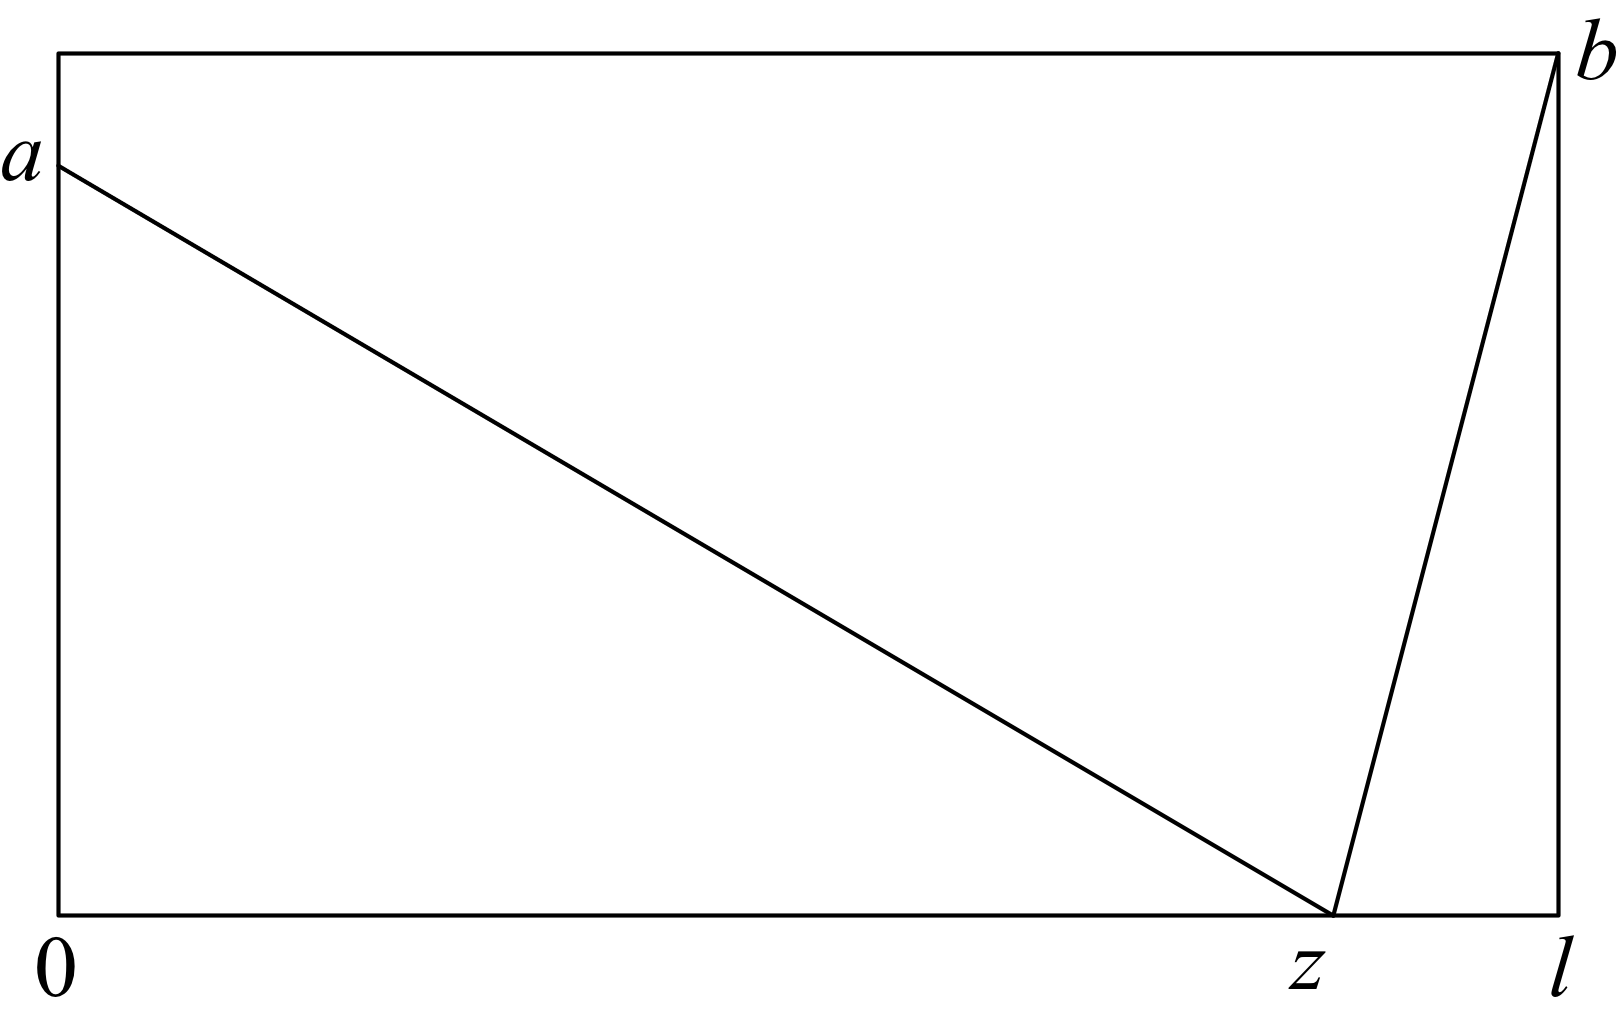
\includegraphics[width=3in]{img/trap.png}
    \caption{Trap function.
    }
    \label{fig:trap}
\end{figure*}


Each local GA had the following parameters, the initial population was randomly generated
with a random size between 128 and 256 individuals, the period to send individuals to the server
was set at 100 local generations, the parameters for the trap function are $l$ = 4,
$a$=1, $b$ = 2, $z$=3 with a chromosome length of 160 bits.


We made a call to participation on November 23th,
2016 through the authors' social networks: ``Asking again for your help, we are conducting a computational experiment
that requires computer power. Can we borrow some of your CPU? just visit the web page (link)
and leave the tab open. Be part of the TOP TEN, register so we can track your participation.
The experiment will run until November 27th, Thanks!.'' As you can
see, the message mentioned a deadline; a link that could be used to
register was also included. Users visiting the page after the deadline
were presented with a thank you message and a final leader
board. Considering the number of friends, followers and the organic
sharing of the posts, we estimate the post was visited by around 2000
users. Only some of them registered, but in fact relatively small samples of users ($10\pm$) are sufficient for
discovering 80\% of usability problems \cite{Schmettow2012}. In fact,
we were not so much interested in making a precise model but on how
the behavior of the registered users was different from non-registered
ones; in non-parametric comparisons, using 15 sample units is in general
good enough, as seems to be the case in this particular
experiment, where we were also interested in computing the number of
users who actually registered, proving that, in fact, for most users
the fact that they have to register represents a bigger effort they
seem to be able to muster for this kind of experiments. 


\subsection{Results}
\label{sec:results}

\begin{table}[h!tbp]
  \small
  \caption{ Log file record structure}
  \label{tab:record}
  \centering
  \small
  \begin{tabular}{l  l}
    \hline\noalign{\smallskip}
    Attribute & Value \\
    \noalign{\smallskip}\hline\noalign{\smallskip}
    chromosome   & The individual sent to the server as a string of 160 bits.  \\ \hline
    fitness & fitness as an integer.  \\ \hline
    IP & IP address of the participant (later anonymized) .\\ \hline
    user & user-name or the string `anonymous'.  \\ \hline
    worker\_uuid & unique identifier of the HTTP Worker that sent the participation.   \\ \hline
    level &  level of user or the string `info' \\ \hline
    message & Only PUT messages were recorded in this experiment. \\ \hline
    timestamp & A time-stamp based on the Unix epoch\\ \hline
  \end{tabular}
\end{table}
%
At the end of the experiment the resulting log file (whose fields are shown in Table \ref{tab:record}) contained 933,513 contributions both
registered users and anonymous volunteers. Registered users were responsible for about
90\% of the contributions, while being only 16\% of the total number of unique users (assuming each IP is from a single user).
The JSON data recorded for each contribution is  presented
in Table~\ref{tab:record}.

\begin{figure}[h!tb]
    \centering
        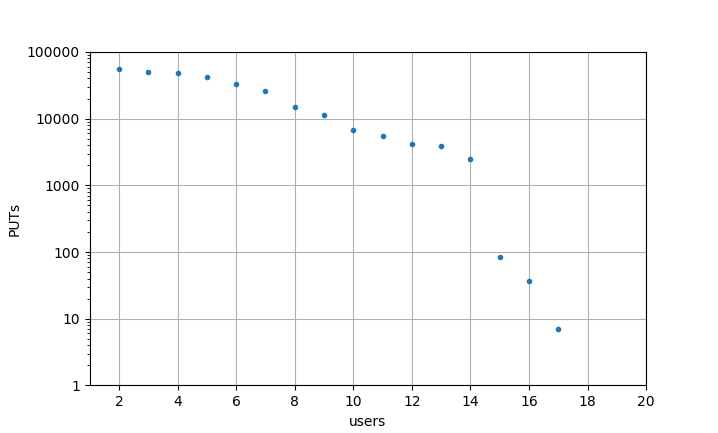
\includegraphics[width=0.9\linewidth]{img/puts_user.png}
        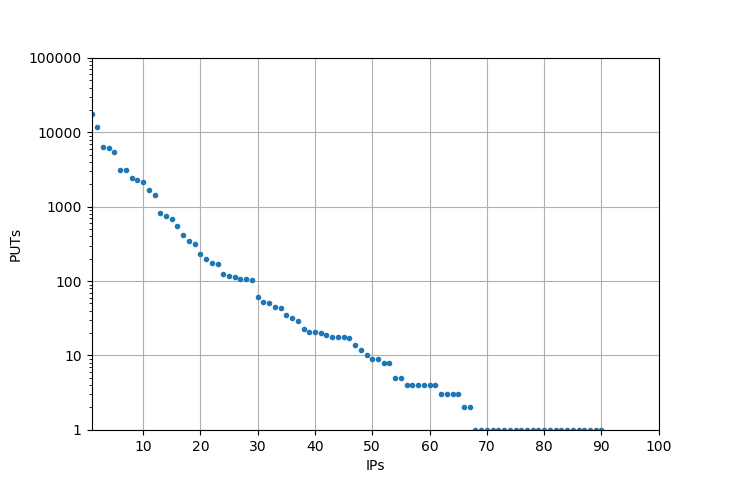
\includegraphics[width=0.9\linewidth]{img/puts_ip.png}
    \caption{Usage by registered (top) and anonymous (bottom) users.  Users are ranked by
        the number of requests sent, in the \emph{x} axis is the rank, and in the \emph{y} axis
        number or PUTs in a logarithmic scale.}
      \label{fig:puts}
% Maybe we should scale dividing by number of users and put them
% together. - JJ
\end{figure}
%
Contributions are expressed as the number of HTTP {\tt PUT} requests
sent to the server. In Figure~\ref{fig:puts} a comparison between the
contribution of registered vs anonymous users is 
presented.

The first observation arises from the length of the $x$ axis. There
were only 18 registered users vs 91 distinct IPs; the 
exact number of anonymous users is upper-bounded by that amount but is
not known precisely as we only recorded the IP of the request, we did
not use cookies or other means of identification since it was not
actually needed for the experiment. Besides, a registered user
could sometimes be anonymous too, which could be caused by the fact that the first time they visited
the application they automatically begin to work as anonymous, so the
number of non-anonymous users, 91, is actually the amount of unique
IPs that had `anonymous' as the user. In the plot of 
anonymous users, some of the last in the rank could in fact be registered users,
momentarily participating as anonymous. Even if this is not considered, only
about 16\% of users attending the call decided to participate as named
users and thus enter the game dynamics. 

The second observation is apparent in the $y$ axis of Figure
\ref{fig:puts}. There is a notable difference in the amount of
participation between the two groups, and also in the slope of the
plot.  An independent-samples t-test was conducted to compare participation, and there was a significant difference in the scores for anonymous users  (M=1057.97, SD= 3669.86) and non-anonymous users (M=46513.55, SD=93537.20); t-test= 4.70, p = 7.5e-06. 

%Maybe a statistical comparison? Median, for instance - JJ
%count          mean           std  min      25%      50%      75%   
%category                                                                     
%IP        91.0   1057.978022   3669.862398  1.0     1.50     18.0    173.0   
%user      18.0  46513.555556  93537.207948  7.0  3962.75  13034.5  46993.5   

           
%      max  
%category            
%IP         26593.0  
%user      396081.0  
%Ttest_indResult(statistic=4.7070787365897289, pvalue=7.565505602664807e-06)
%

\begin{figure*}[htb]
    \centering
        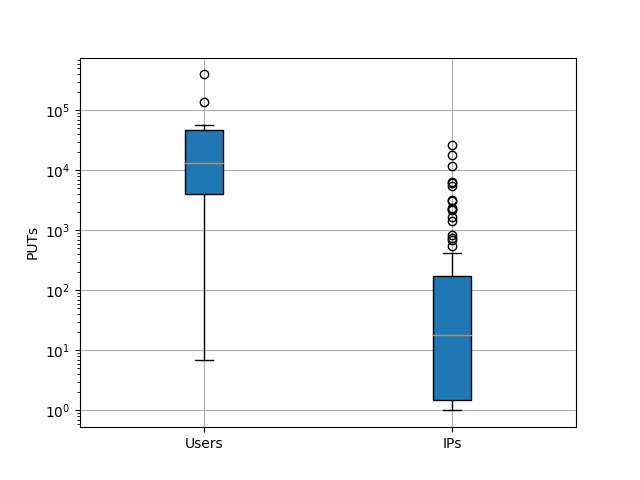
\includegraphics[width=5in]{img/puts_box.png}
    \caption{ Box-plot of the number of requests sent by registered users and anonymous IPs.
     In the \emph{y} axis are number or PUTs in a logarithmic scale.
    }
    \label{fig:box}
\end{figure*}
%
The box plot featured in Figure \ref{fig:box} shows the amount of participation between the two groups, it highlights
the difference and also the number of outliers in the groups. Two registered
outliers were very important participants, maybe competing between them. But
there were more outliers between anonymous IPs, and some of them could be related to the same users. The lower quartile in the users box-plot has more
spread, indicating a participation similar to the median of anonymous IPs.

%
\begin{figure*}[htb]
    \centering
        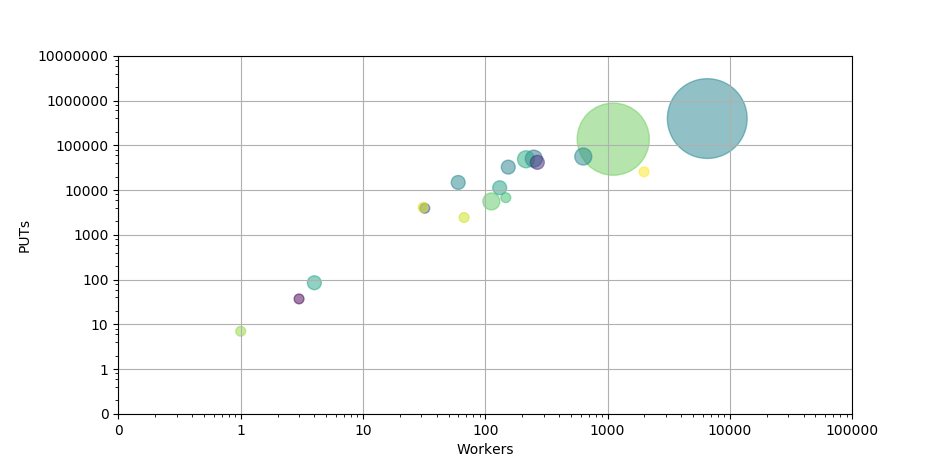
\includegraphics[width=5.3in]{img/workers_put_ip.png}
    \caption{ Participation of registered users. Each circle represents a user relating
        in the \emph{x} axis the number of workers used and in the \emph{y} axis
        number or PUTs in a logarithmic scale. The area of the circle is the number
        of unique IPs used by the user.
    }
    \label{fig:worker-put-ips}
\end{figure*}
%
Figure~\ref{fig:worker-put-ips} gives an interesting view on the amount of
resources shared by registered users. The area of the circle is proportional
to the number of unique IPs used by each user, the user with more participation
used a total of 66 different IPs, this number could be related with the number
of devices used during the participation. There are some users that using less
devices participated more, this could mean a more powerful device, faster
Internet connection or simply more time spent participating.

\begin{figure*}[htb]
    \centering
        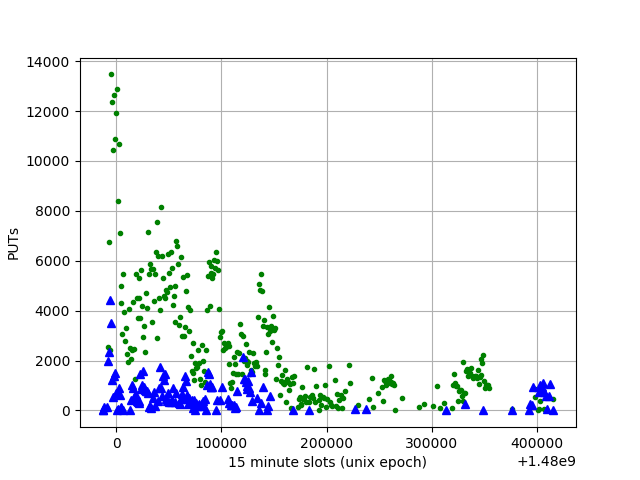
\includegraphics[width=5.3in]{img/puts_by_time.png}
    \caption{Number of PUTs by User (green dots) or IP (blue triangles) in 15 minute slots.
    }
    \label{fig:puts-time}
\end{figure*}
%
User engagement is related to the amount of time a user spends in the
application. Figure~\ref{fig:puts-time} shows two important aspects of
engagement, the overall time spent and the amount of resources shared
in that time. Registered users were more engaged during the experiment.
They contribute more resources during longer periods of time.

\begin{figure*}[htb]
    \centering
        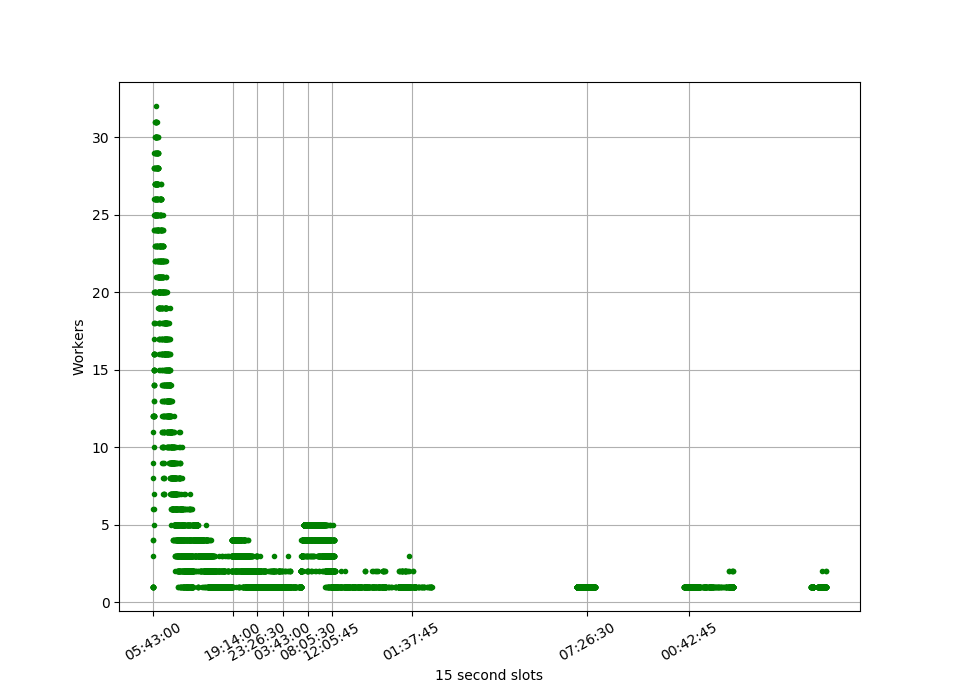
\includegraphics[width=5in]{img/workers_best_user.png}
    \caption{ Number of workers used by the top ranked user in 15 minute slots.
    }
    \label{fig:top-user}
\end{figure*}
%
The amount of participation of the top ranked user is presented in 15 seconds time slots in
Figure~\ref{fig:top-user}. In the beginning this user was using more than 30
workers, this means that more than 30 tabs of the page were open at the
same time, perhaps using several computing devices. Some users reported that
they wanted to test the limits of their own systems, checking the percentage of
CPU they were using.

\section{Conclusions, discussion and future work}

The objective of this work was to test the kind of impact
applying a gamification technique has on user engagement in
the Anonymous
% {\sf NodIO}
volunteer computing framework; In concordance with
the results obtained in other
browser-based volunteer systems, after
applying the gamification techniques, user participation was increased.


In this paper we have added gamification to a volunteer computing
system via a leaderboard of contributions of registered users. In
fact, we have proved that, although only a minority of the users opt
for registration, their individual contribution is on average much
higher than for non-authenticated/non-gamified users. The fact that less
than one fifth of users opt for registering would discard the
exclusive use of this feature; however, it is an interesting addition
to the volunteer system that in fact enhances its computing power.

The fact that gamification actually work highlights the social nature of volunteer computing systems, piling on the fact that successful {\em social clouds} must embed games and other social mechanisms to enhance participation. That is why future lines of work will look for intermediate ways of including
gamification without registration, as well as some ways of making the
user increase control over the algorithm that would go beyond simply
staying for longer or leaving the page. Since it is a sociotechnical
system, including social features in it and studying emerging social
networks is an interesting line of work too.

Other factors, such as the language used, the way the experiment is announced, are also very important in this social context, which is why they will be included in future lines of work too.

One of the interesting future lines of work would be to look a bit
more closely at the behavior of users as they are participating
in the web system.

Another line of work would be to study the possible negative effects of using
gamification techniques to improve engagement, like cheating or
literally {\em gaming} the system to defeat competition. We already
found some hints of this behavior, but more subtle effect could be taking place.
Finally, the refinement of the proposed framework will need
more case studies and further multi-disciplinary research.


\section*{Acknowledgments}

% This work has been supported in part by: Ministerio espa\~{n}ol de
% Econom\'{\i}a y Competitividad under project TIN2014-56494-C4-3-P
% (UGR-EPHEMECH).
Hidden for double blind.


\bibliographystyle{splncs03}

\bibliography{../../bib/biblio,../../bib/evospace-i,../../bib/volunteer,../../bib/geneura}

\end{document}
